\section{Implementation}
\label{implementation}

The first CTFE First was created for the C-=-1 language, using out-of-the-box parser generator and backend.

\subsection{Interpreter data structures}

Data structures of the C-=-1 Interpreter have been designed ease of development and debugging in mind.
They are thus not particularly efficent.

\begin{figure}
	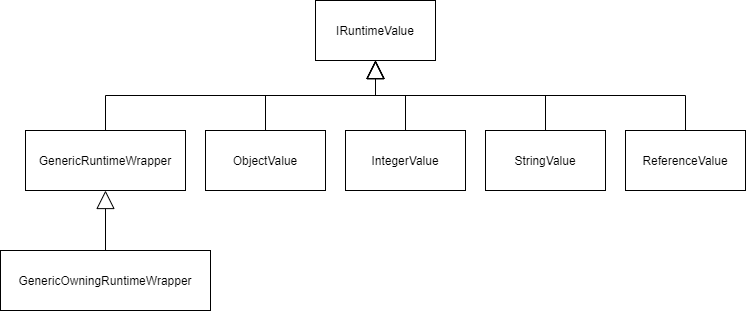
\includegraphics[width=8cm]{pictures/interpreter_data_structures_uml.png}
	\caption{Class diagram of C-=-1 interpreter data structures}
	\label{fig:interpreter_data_structures}
\end{figure}

Figure \ref{fig:interpreter_data_structures} contains a class diagram of most of the types used to represent values within C-=-1.
All of them derive from \lstinline{IRuntimeValue} and are managed via C++ smart pointers.
The interface of the base class allows the value to be converted to a human readable format, serialisation, deserialisation and copying.

The most prymitive types within the hierarchy are \lstinline{StringValue} and \lstinline{IntegerValue}.
They are simple wrappers for strings and integers.
Floating point numbers were not implemented as they were not nessecary for implementation of a basic compiler.

User-defined types are represented using \lstinline{ObjectValue}.
The contents of an objects is kept as a \lstinline{string} - \lstinline{IRuntimeValue} dictionary, with field names as keys and \lstinline{uniqe_ptr<IRuntimeValue>} as values.
C-=-1 object is therefore spread out in memory, even if the fields are directly contained within the class, without any indirection.

There are multiple types of reference within the C-=-1 interpreter.
The most basic pointer type is a reference to C-=-1 value.

\subsection{Program semantic model}

\subsection{Backend interface}
\label{implementation/backend-interface}
